\chapter{Informality and Development}

\fancyhead[L]{ECON0024}
\fancyhead[C]{Ch.5 Informality and Development}
\fancyhead[R]{Xiaotian Tian}
\fancyfoot[L]{\hyperlink{tableofcontents}{Back to Table of Contents}}
\fancyfoot[R]{Xiaotian Tian}


\section{Basics and Facts}
    \subsection{Definitions}
        \subsubsection{Legalistic Definition}
        
            Informal firms and workers are those that \empha{operate at the margin of the relevant laws and regulations}. This excludes obviously illegal activities, such as drug smuggling, but includes unregistered/tax-evading firms.
            
            We do NOT define informality by sizes.
            
        \subsubsection{Two Margins of Informality for Firms}
            \begin{enumerate}
                \item \emphb{Extensive Margin}: whether to register the business
                \item \emphb{Intensive Margin}: whether registered firms hire informal workers (or not comply with taxes)
            \end{enumerate}
            For employees, there's only one kind of informality: whether employed informally or not.
            
    \subsection{Statistical Facts}
        Informal firms occupy a share around 70\% in Brazil (extensive margin); informal workers have a share of 30-80\% of the labour force in Latin American countries (either employed by informal firms (extensive margin) or employed informally by formal firms (intensive margin)). Specifically, the intensive margin accounts for 40-44\% of informal employment in LAC.\par
        \begin{itemize}
            \item Informality is pervasive
            \begin{figure}[H]
                \centering
                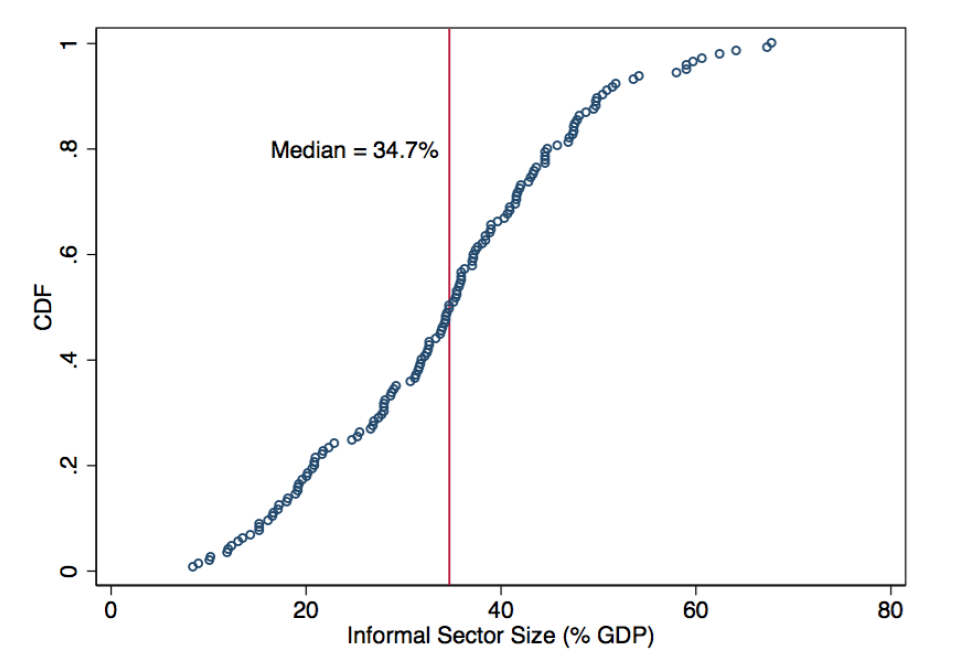
\includegraphics[width=4in]{images/ch5/pervasive_informality.png}
                \caption{Distribution of Informal Sector Size as \% of GDP}
            \end{figure}
            \item Informality is negatively correlated with GDP per capita
            \begin{figure}[H]
                \centering
                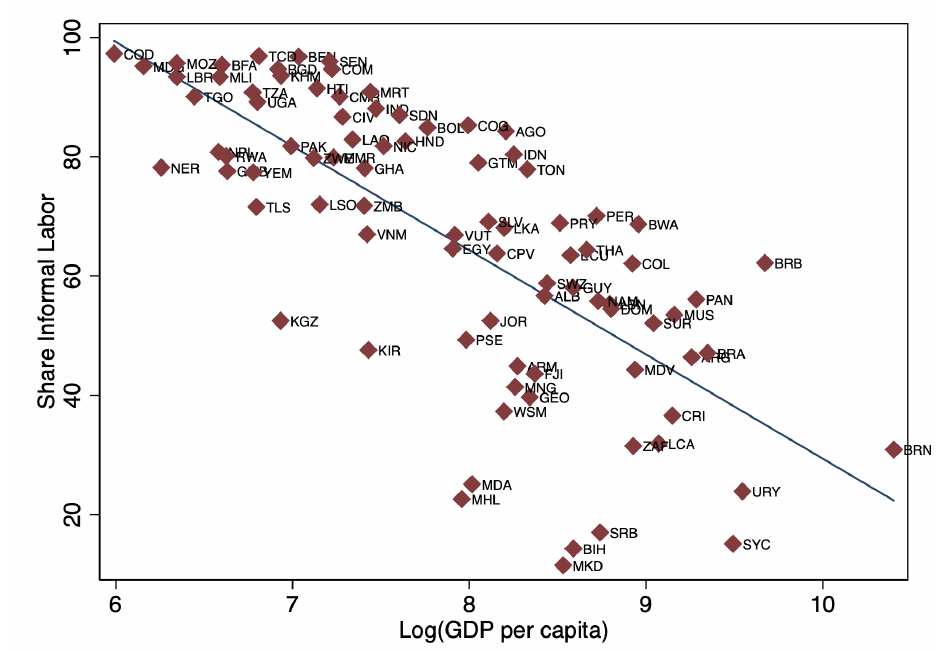
\includegraphics[width=4in]{images/ch5/informality and gdp.png}
                \caption{Share of Informal Labour against Log GDP per Capita}
                \label{fig:informality_gdp}
            \end{figure}
            \item There are huge variations of informality even within income groups
            \begin{figure}[H]
                \centering
                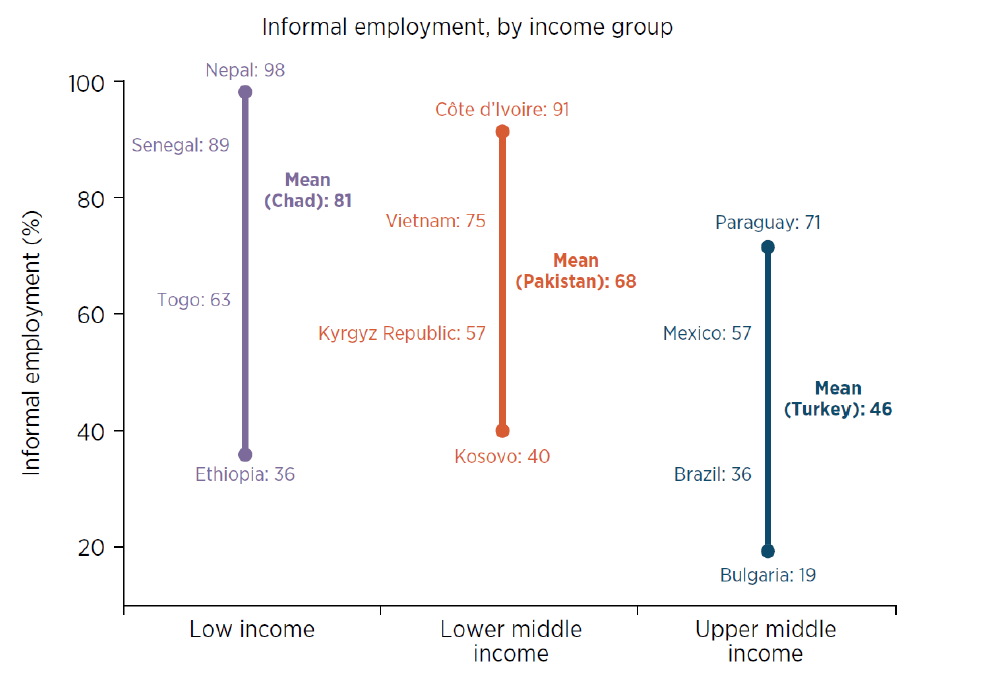
\includegraphics[width=4in]{images/ch5/variation within income groups.png}
                \caption{Variations within Income Groups (\cite{penny_goldberg_penny_2022})}
            \end{figure}
            \item Despite the negative correlation found in fig \ref{fig:informality_gdp}, economies cannot simply \emphb{grow out of informality}. In the graph below, economies coloured light grey have shrinking informal sectors as they grow. However, on the other hand, economies coloured black have stable/expanding informal sectors as they grow. A representative case is India (coloured red): despite fast growth and development, its informal sector has hardly diminished. (Note that informality reduction itself should not be considered as an economic goal because its welfare implication is ambiguous.)
            \begin{figure}[H]
                \centering
                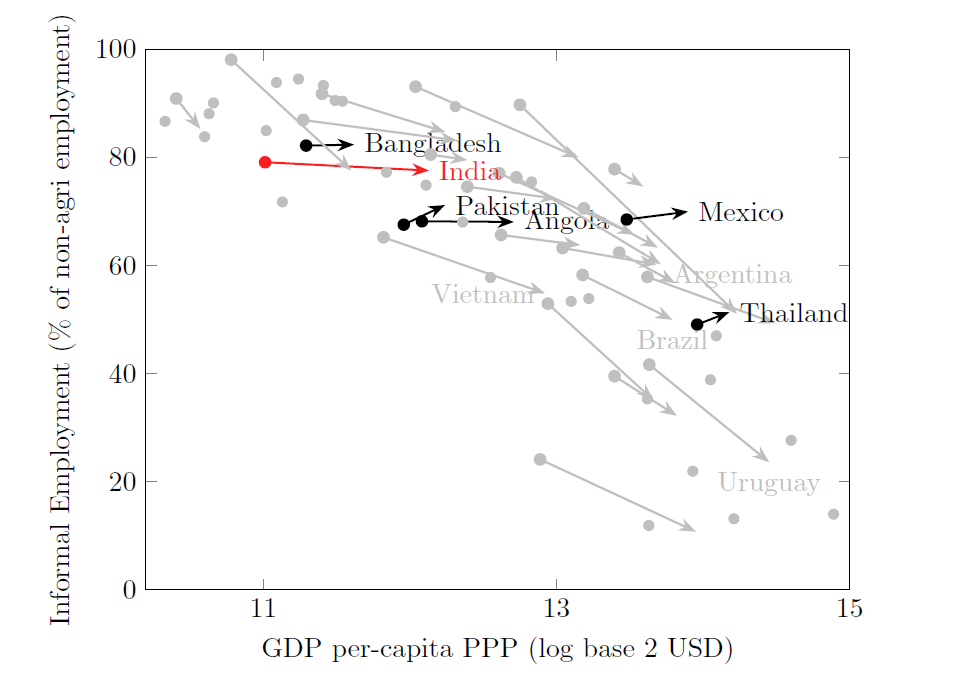
\includegraphics[width=4in]{images/ch5/cant grow out of informality.png}
                \caption{Trajectory of Informal Employment (Belavadi, 2021 (PhD Thesis, Penn State))}
            \end{figure}
        \end{itemize}
        
    \section{Formal vs. Informal Firms: No Duality and Dynamics}
            Informal firms are on average smaller, pay lower wages, have less educated owners, hire less educated employees, and earn lower profits.
            
            \subsection{Lack of Duality}
                 Nevertheless, differences above do not necessarily indicate a \emphb{dualistic view}. Formal firms and informal firms \empha{coexist} within narrowly defined industries, and there is a substantial overlap in the productivity distribution of formal and informal firms, even within industries:
                \begin{figure}[H]
                    \centering
                    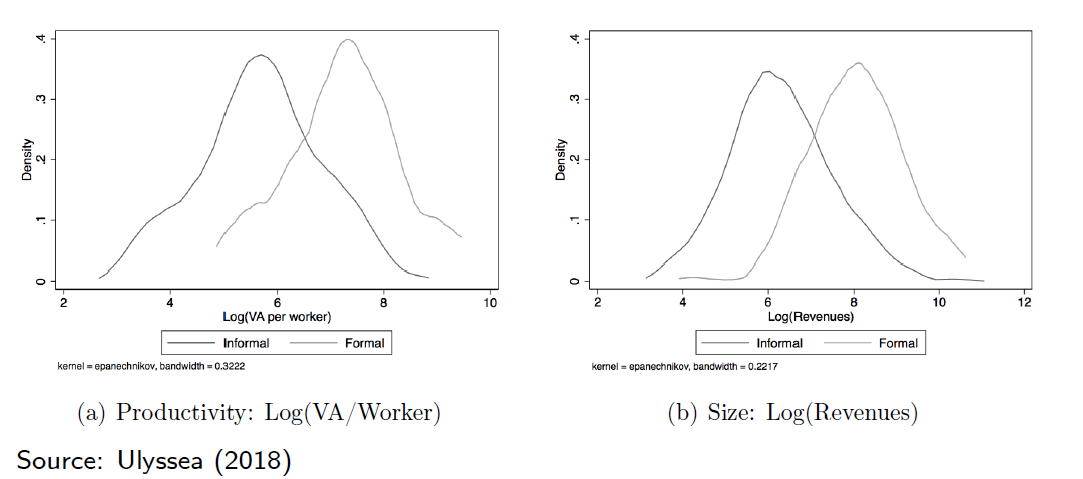
\includegraphics[width=5.5in]{images/ch5/duality.png}
                    \caption{Large Overlap in Sizes/Productivity Distributions (\cite{ulyssea_firms_2018})}
                \end{figure}
            
            \subsection{Missing Middle?}
                \emphb{Missing middle} refers to situations where there are a large number of firms with either a few employees or many employees, with a thin distribution in between. Missing middle is an indication for economic solidification, which is harmful for growth and development.
                
                The distribution of firms does not shown a "missing middle." Both extensive and intensive margins of informality are negatively correlated with firm sizes:
                \begin{figure}[H]
                    \centering
                    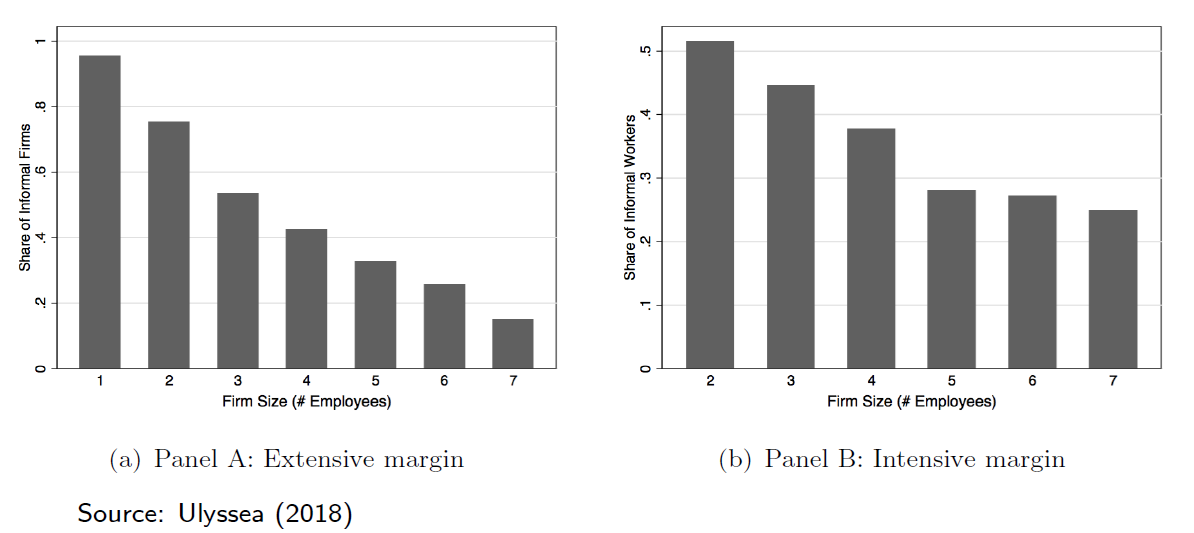
\includegraphics[width=5.5in]{images/ch5/margins of informality and sizes.png}
                    \caption{Margins of Informality and Firm Sizes - Brazil (\cite{ulyssea_firms_2018})}
                \end{figure}
                However, there is a missing middle in employment distributions:
                \begin{figure}[H]
                    \centering
                    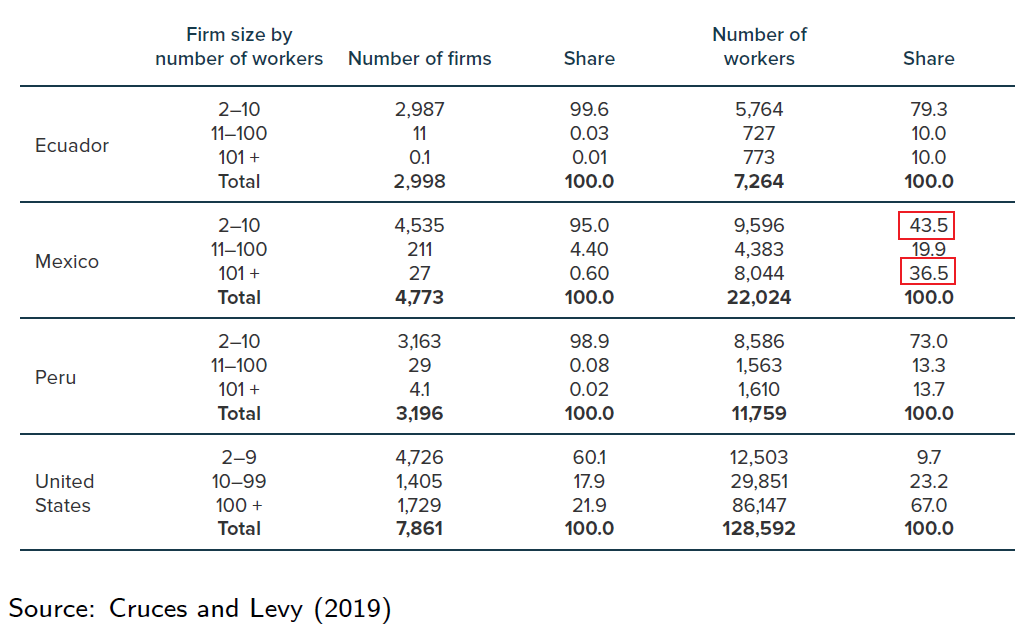
\includegraphics[width=5.5in]{images/ch5/missing middle emp 1.png}
                    \caption{Missing Middle in Employment - Mexico}
                \end{figure}
                \begin{figure}[H]
                    \centering
                    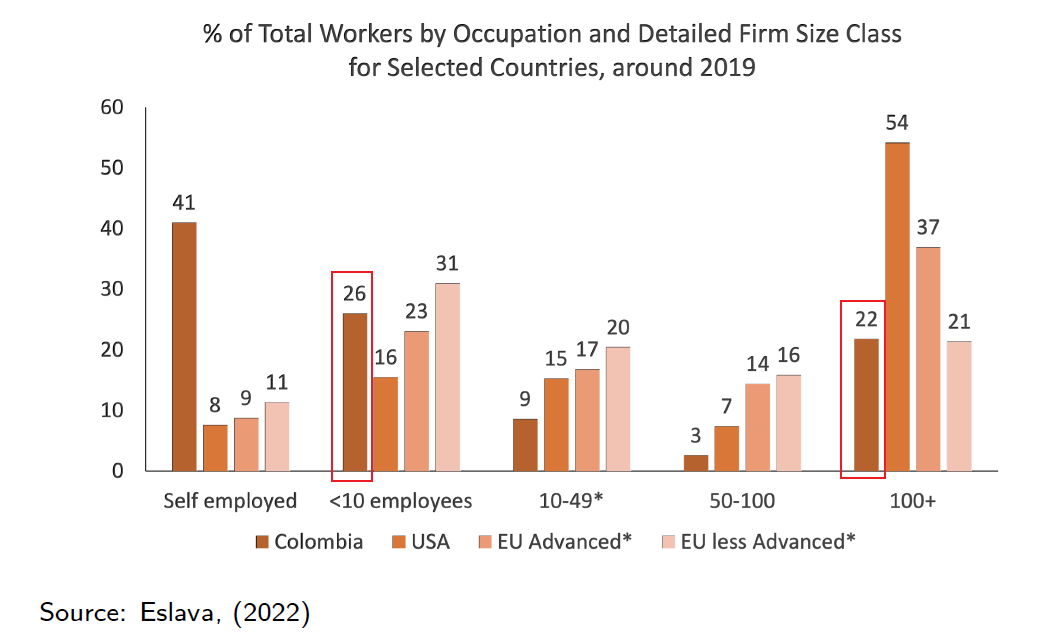
\includegraphics[width=4in]{images/ch5/missing middle emp 2.png}
                    \caption{Missing Middle in Employment - Colombia}
                \end{figure}
                
            \subsection{Informality and Firm Expansions}
                Overall, evidences show us that firms in developing countries \empha{grow less} and \empha{stagnant firms survive longer}:
                \begin{figure}[H]
                    \centering
                    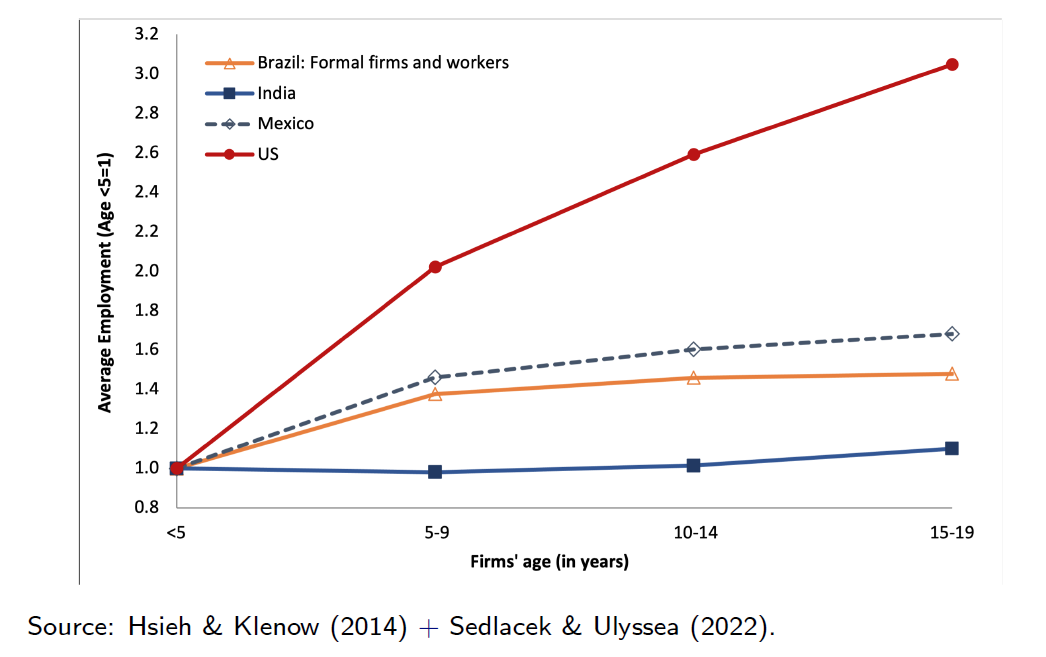
\includegraphics[width=4in]{images/ch5/dynamics_1.png}
                    \caption{}
                \end{figure}
                \begin{itemize}
                    \item The red line represents U.S.: its high gradient shows that surviving firms in U.S. expand very fast, and some small firms quickly die out
                    \item On the other hand, the dash line represents India: expansion of firms is stagnant (maybe due to the family/gender business traditions)
                    \item The orange line represents the formal sector in Brazil: if the informal sector is included, it will be approximately the same as India
                \end{itemize}
                One explanation for such stagnation could be \empha{related to informality}: as shown in the following figures, there is a positive correlation between entry rate and informality: plenty of firms enter the market as informal ones; on the other hand, those new entrants tend to expand very slow as firms' growth rate is negatively correlated with informality.
                \begin{figure}[H]
                    \centering
                    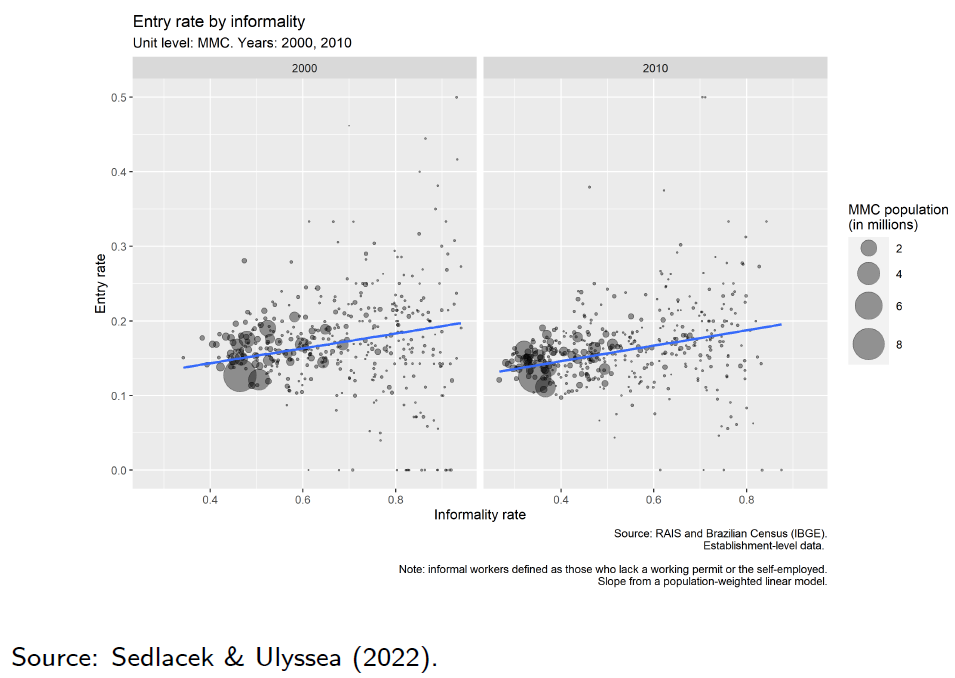
\includegraphics[width=2.9in]{images/ch5/dynamics_2.png}
                    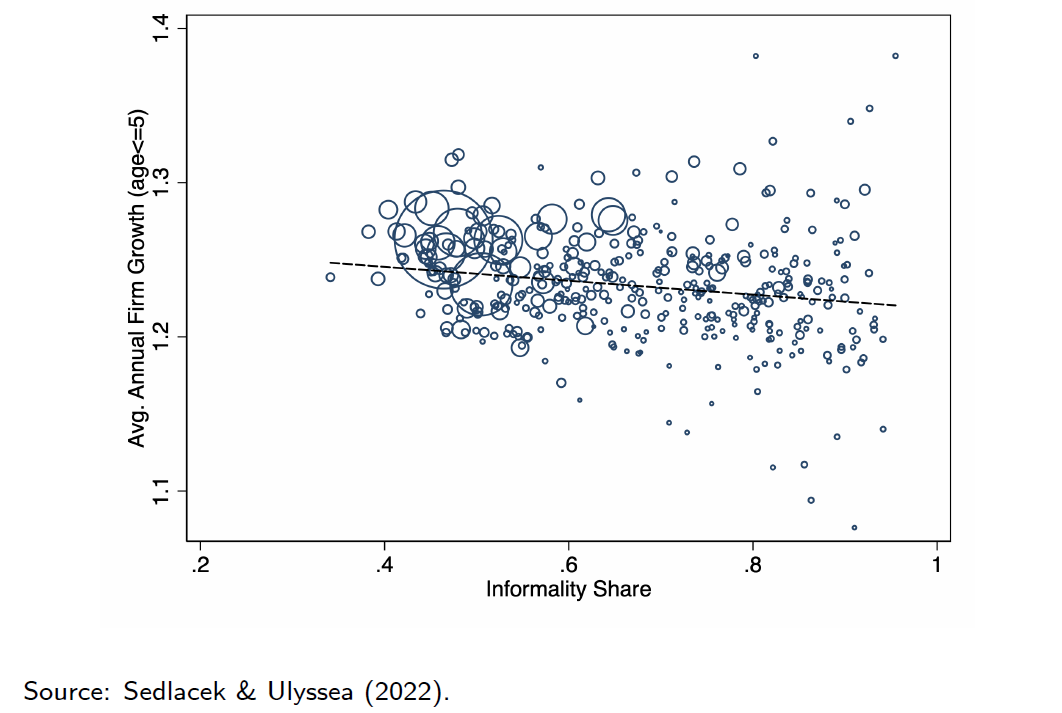
\includegraphics[width=2.9in]{images/ch5/dynamics_3.png}
                    \caption{Left: Entry Rate and Informality; Right: Firm Growth and Informality}
                \end{figure}
                In addition, we also have evidences that:
                \begin{itemize}
                    \item Firms' average sizes increase with their ages, in both formal and informal sectors
                    \item Extensive and intensive margins of informality decrease with firms' age
                    \item A substantial fractions of informal firms eventually formalise
                \end{itemize}
                
            \subsection{Employees' Perspective: Wage Gaps \& Income}
                Considering all workers as a whole, there is no significant overall effect of informality on wages after controlling firm fixed effects. (Red boxes)
                
                For unskilled workers, being employed in the formal sector significantly increase their wages. However, for skilled workers, no such effect is observed. The reason behind this difference could be that the minimum wage becomes binding for the unskilled workers as they become formally employed. (Orange boxes)
                \begin{figure}[H]
                    \centering
                    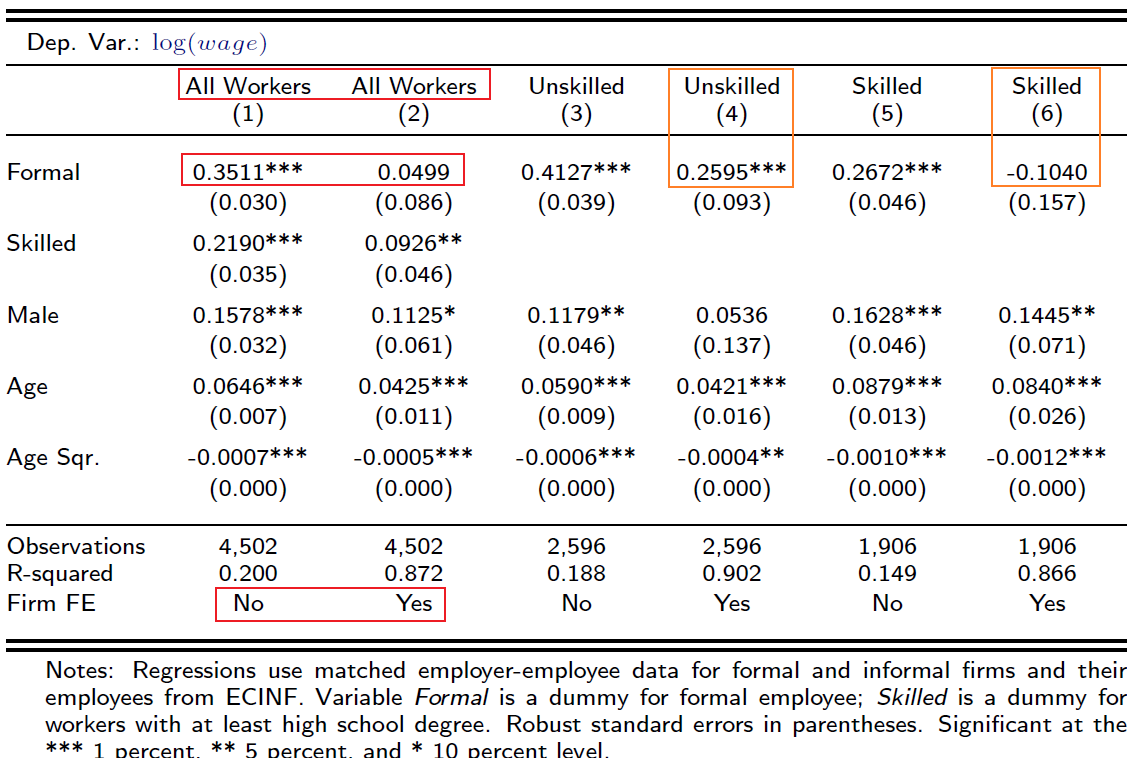
\includegraphics[width=5in]{images/ch5/wage gaps.png}
                    \caption{Log Wage Regression on Formal Dummies and Controls}
                \end{figure}
                Hardly surprisingly, we also have evidence that labour informality is negatively correlated with household income:
                \begin{figure}[H]
                    \centering
                    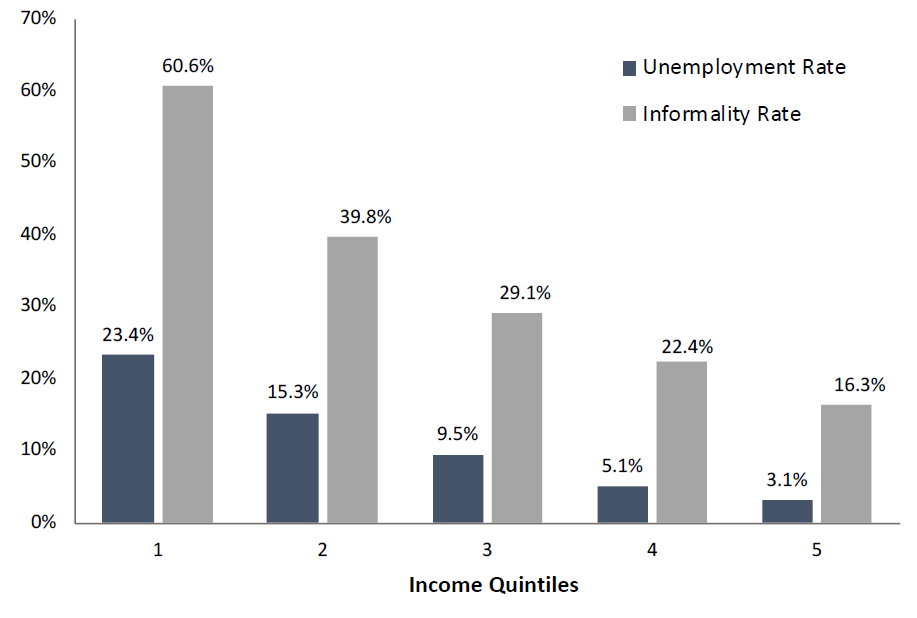
\includegraphics[width=4in]{images/ch5/informality and income.png}
                    \caption{Labour Informality and Household Income}
                \end{figure}
            
            \subsection{Transfer Into and Out of Informality}
                Hiking unemployment in the 90s sheds light on the patterns of employment in both formal and informal sector:
                \begin{figure}[H]
                    \centering
                    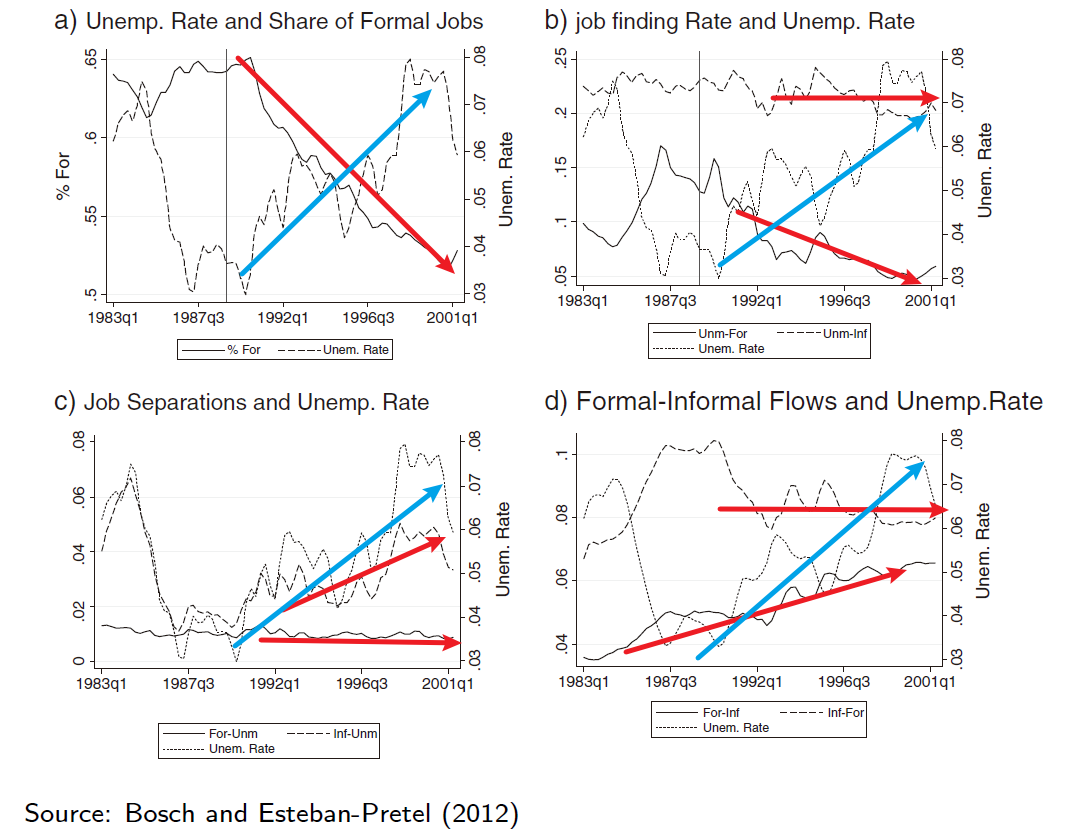
\includegraphics[width=5.5in]{images/ch5/ins and outs of informality.png}
                    \caption{Transfer Into and Out of Informality (\cite{bosch_job_2012})}
                \end{figure}
                \begin{itemize}
                    \item Graph a: informality is \empha{counter-cyclical}: when there is a recession, the informal sector occupies a higher share in the economy, providing a potential buffer
                    \item Graph b: this shows the probability with which workers find formal/informal jobs from unemployment, and it corroborates graph a: during the recession, it becomes harder to find a job in the formal sector while the job finding rate in the informal sector remains unchanged.
                    \item Graph c: during the recession, job separation (destruction/layoff) increases clearly, indicating worse job security in the informal sector, since there is no firing cost
                    \item Graph d: direct transitions from informality to formality are procyclical (easy to see from graph) as they correlate negatively with unemployment rate; Direct transitions from formality to informality are also procyclical (less easy to see) but less volatile
                \end{itemize}
                Overall, we can conclude that the main reason why informality is counter-cyclical is not because of the flow between formal and informal jobs, but the flow between unemployment and formal/informal jobs.
            
\section{$\star$ Modelling Informality}
    \subsection{Model Setup}
        For now, we focus on the \emphb{extensive margin} only.
        Operating \emph{formally}, firms' profit function can be expressed as:
        $$\color{red} \pi_f(\theta) = (1-\tau_y)\underbrace{\theta F(k,l)}_{\equiv y(\theta)} - (1+\tau_w)w_fl -r_f k - \bar{c}_f$$
        Operating \emph{informally}, firms' profit function can be expressed as:
        $$\color{red} \pi_i(\theta) = \Big[1-p\big(y(\theta)\big)\Big]\theta F(k,l) - w_il -r_ik$$
        where:
        \begin{itemize}
            \item $\tau_y$ is the revenue tax rate
            \item $\theta$ represents firm's productivity
            \item $\tau_w$ is the payroll tax rate
            \item $F(.)$ is the production function, increasing and concave in $l$ and $k$
            \item $w_f, w_i$ are formal/informal wages (usually assume $w_f>w_i$)
            \item $l$ is the amount of labour employed
            \item $r_f, r_i$ are capital rents (usually assume $r_f<r_i$ because formal firms have access to more loans and are considered less risky)
            \item $k$ represents capital used
            \item $p(y(\theta))$ represents the "cost of informality," increasing and convex in firm's output $y$
            \item $\bar{c}_f$ is the per-period fixed cost that only formal firms must pay
        \end{itemize}
        Note that, in addition to those costs, formalisation of a firm must incur in a \emphb{fixed registration cost}, which varies dramatically across countries.
    
    \subsection{Policy Implications}
        Our model shows us that policymakers can incentive firms to formalise by:
        \begin{itemize}
            \item Reducing costs of formality: costs of entering the formal sector (registration) and costs of remaining formal (e.g. taxes)
            \item Increasing the benefits of formality: e.g. more access to capital (lower $r_f$)
            \item Increasing the costs of informality: e.g. higher enforcement of existing laws and regulations
        \end{itemize}
        
\section{Empirical Evidence and Interpretation}

    \subsection{Evaluation of Treatments to Facilitate Formalisation}
        \subsubsection{Regression setting}
            \begin{equation}
                y_{it}=\alpha+ \beta \text{Treatment}_{it} +\gamma X_{it}+\epsilon_{it}
                \label{eqn:formality regression 1}
            \end{equation}
            \begin{itemize}
                \item Unit of analysis ($i$): typically firm or entrepreneur
                \item $y_{it}$: formality dummy or share of formal firms
                \item $\text{Treatment}_{it}$: formalisation treatment dummy (=1 if treated)
                \item $X_i$ is a vector of Controls
                \item ATE is identified ($\beta_{OLS} = E[Y_{1i}-Y_{0i}]$) under the assumption: $(Y_{1i},Y_{0i}) \perp D_i|X_i$ because there is no selection on levels/gains conditional on $X_i$.            
            \end{itemize}
        \subsubsection{Results}
            \begin{figure}[H]
                \centering
                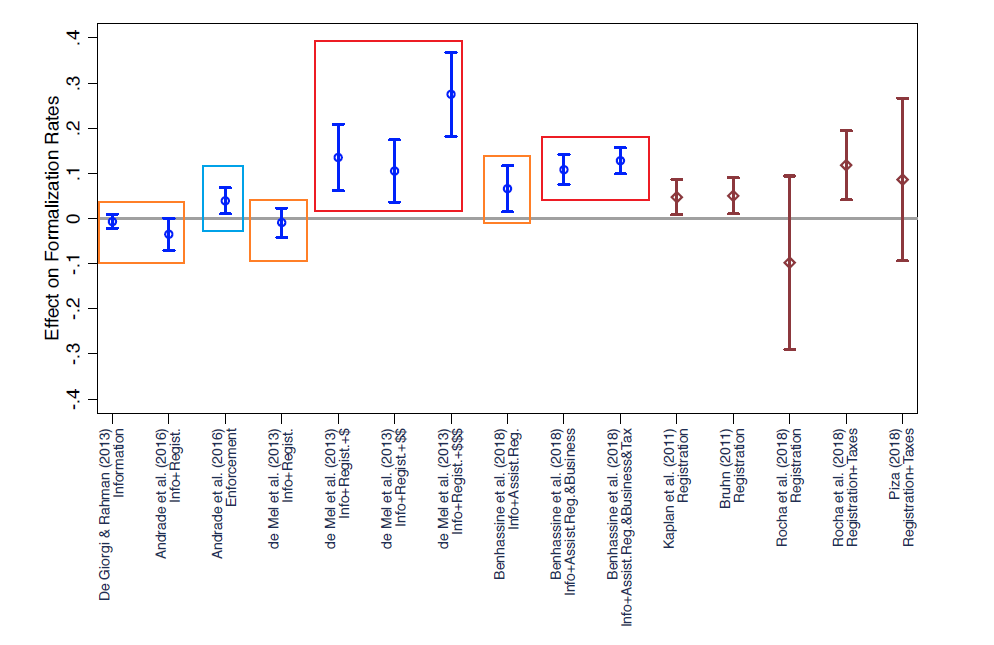
\includegraphics[width=5in]{images/ch5/formal policies evaluation.png}
                \caption{Estimated Effects on Formalisation Rates of Different Formalisation Treatments (\cite{ulyssea_informality_2020})}
            \end{figure}
            \begin{itemize}
                \item Orange squares incorporate treatments that reduce registration costs or provide information, which have no significant effect on formalisation. This reveals that high \emphb{fixed costs} for formalisation may not be the main obstacle.
                \item Red squares incorporates treatments that reduce \emphb{ongoing costs}, which show significant positive effects on formalisation
                \item The blue square incorporates the only paper that studied higher \emphb{enforcement}, whose effect is significant. However, in reality, such intervention may have political economy concerns.
            \end{itemize}
    
    \subsection{Fixed and Ongoing Costs of Formalisation: RCTs in Sri Lanka}
        This paper written by \cite{de_mel_demand_2013} used experiments in Sri Lanka to explore effects of covering registration costs and ongoing costs.
        
        \subsubsection{Research Designs and Treatments}
            \begin{itemize}
                \item Treatment 1: Provide information + Cover direct monetary costs of firm registrations
                \item Treatment 2: Treatment 1 + 10,000 rupees (50\% of median monthly profits)
                \item Treatment 3: Treatment 1 + 20,000 rupees
                \item Treatment 4: Treatment 1 + 40,000 rupees
            \end{itemize}
            Treatment 1 only covers the fixed cost of registration the firm, while treatment 2-4 also provide additional money transfers, which can be understood as compensations for discounted future ongoing costs.
            \begin{figure}[H]
                \centering
                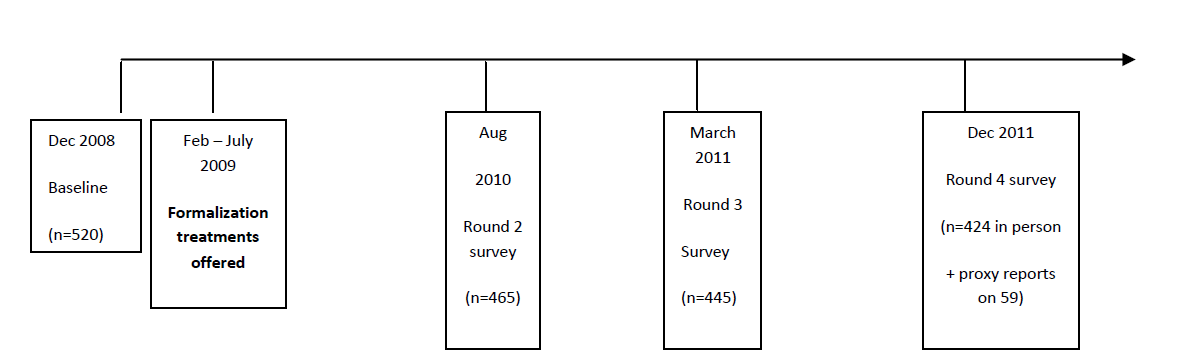
\includegraphics[width=5.5in]{images/ch5/SL formal treatment 1.png}
                \caption{Research Timeline}
            \end{figure}
        \subsubsection{Results: Effects on Formalisation}
            \begin{figure}[H]
                \centering
                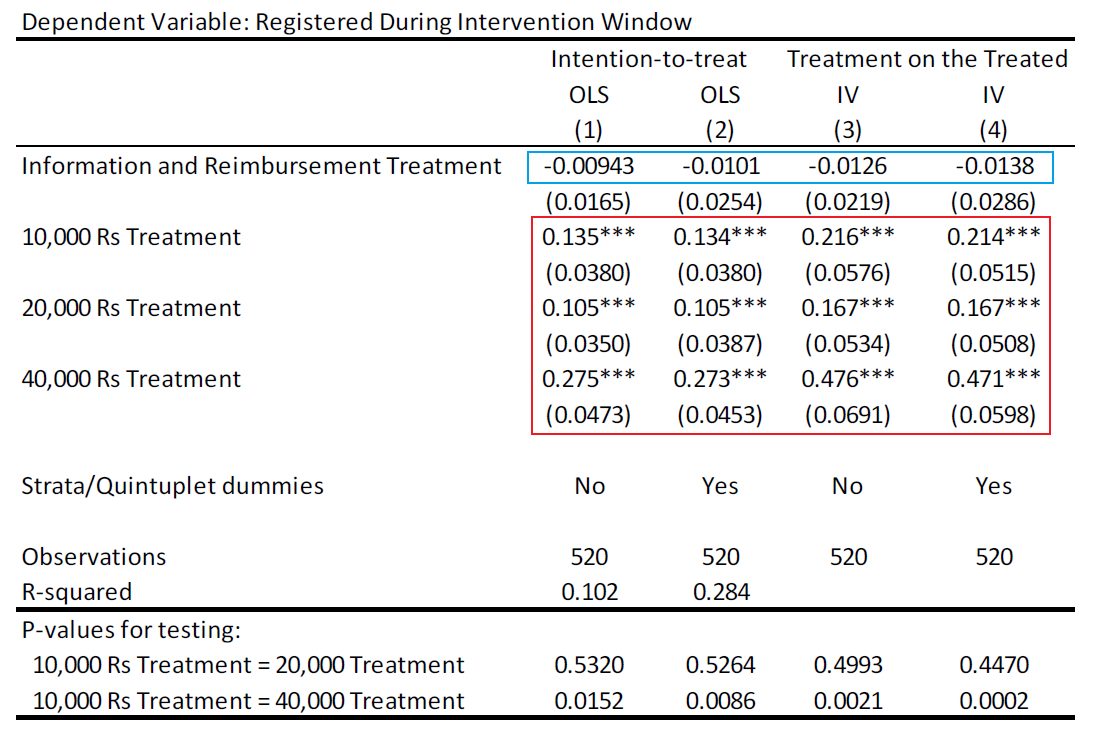
\includegraphics[width=5.5in]{images/ch5/SL formal treatment 2.png}
                \caption{Effects of Treatments on Formalisation}
            \end{figure}
            The figure above shows the Intention-to-Treat (ITT) and Treatment on the Treated (ATT) estimates of corresponding treatment (on the rows). ITT is calculated by directly regressing the formality dummy on the treatment dummy and covariates. ATT is identified as LATE using invitation as an IV for treatment. Put differently, ITT is the treatment effect of assignment while ATT/LATE is the treatment effect on compilers.

            Results indicate that only covering the fixed cost of registration is not enough to induce firms to formalise (ITT/ATT of treatment 1 are not significant). Treatment with additional money to cover ongoing costs are more effective, and their effects increase with the amount of payment, as indicated by figures in the red square.
            
        \subsubsection{Results: Effects of Formalisation on Firms' Performance}
            \begin{figure}[H]
                \centering
                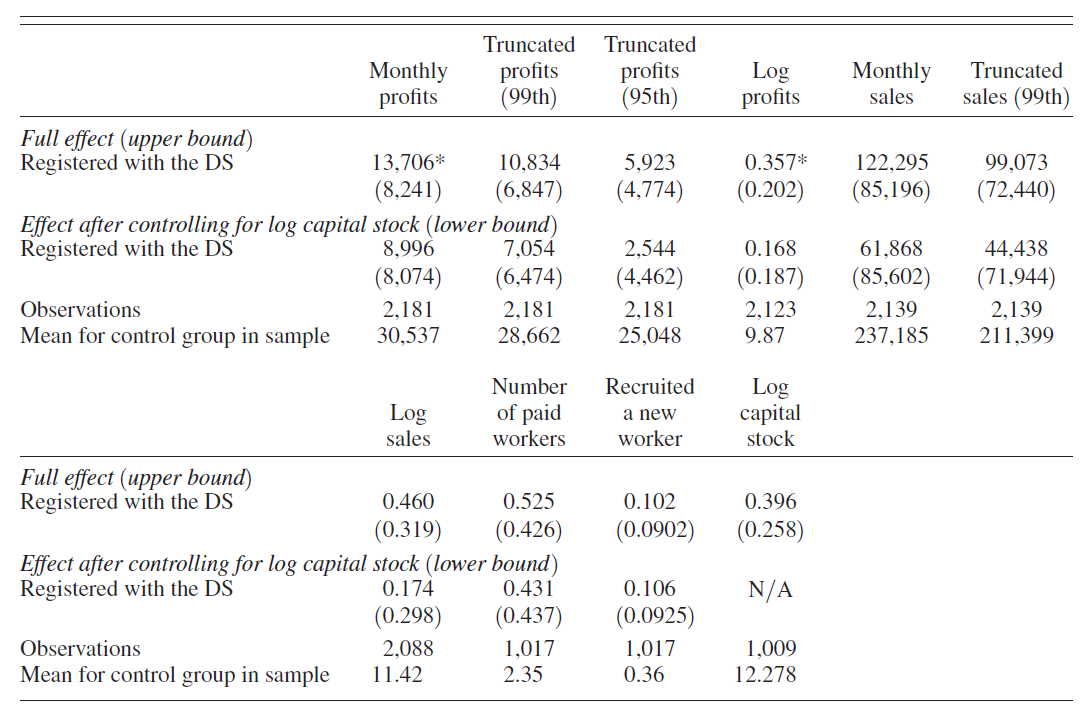
\includegraphics[width=5.5in]{images/ch5/SL formal treatment 3.png}
                \caption{Effects of Formalisation on Firms' Performance}
            \end{figure}
            Using the treatment as an IV for formalisation, Suresh et al. estimated the effects of formalisation on firms' performance indicators. Overall, there is no significant positive effects. This provides insights that \empha{becoming formal may not be beneficial for firms}.
            \begin{figure}[H]
                \centering
                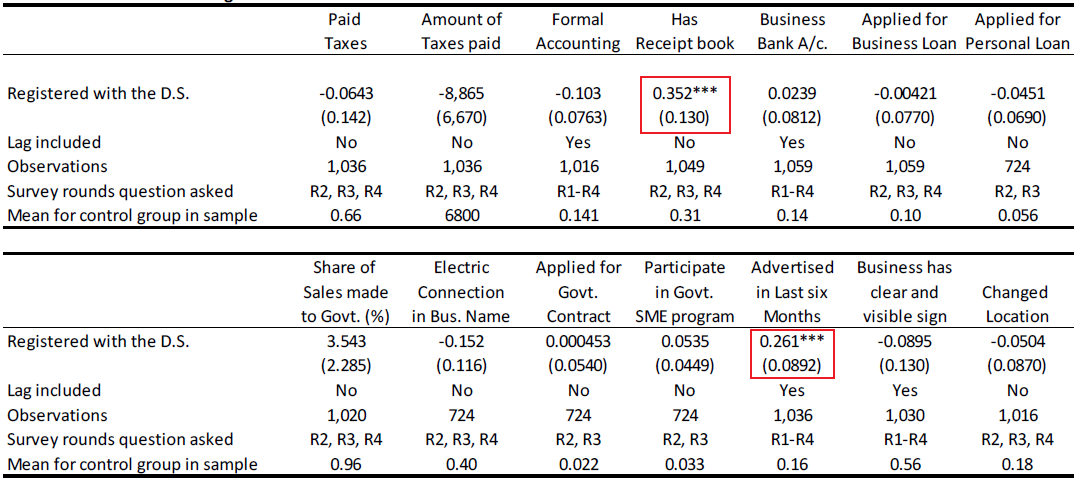
\includegraphics[width=5.5in]{images/ch5/SL formal treatment 4.png}
                \caption{Effects of Formalisation through Different Channels}
            \end{figure}
            Taking a closer look at potential channels through which formalisation could affect firms' performance: we can see that nothing was significantly changed except that now formal firms have receipt books and advertise more.
    
    \subsection{Other Literatures}

        Apart from the literature discussed in the lecture, \cite{de_andrade_helping_2014} also argues that waiving the lump-sum registration fee is not useful in promoting formalisation. They conducted a RCT in Belo Horizonte, Brazil. In one of the treatments, researchers eliminated all registration costs as well as sanitary tax, municipal inspection fee, and accounting service charge for the first year. Results are summarised in figure \ref{fig:rct brazil result} (column named "Free Cost Difference"): results are at best insignificant, at worst negative.

        \begin{figure}[H]
            \centering
            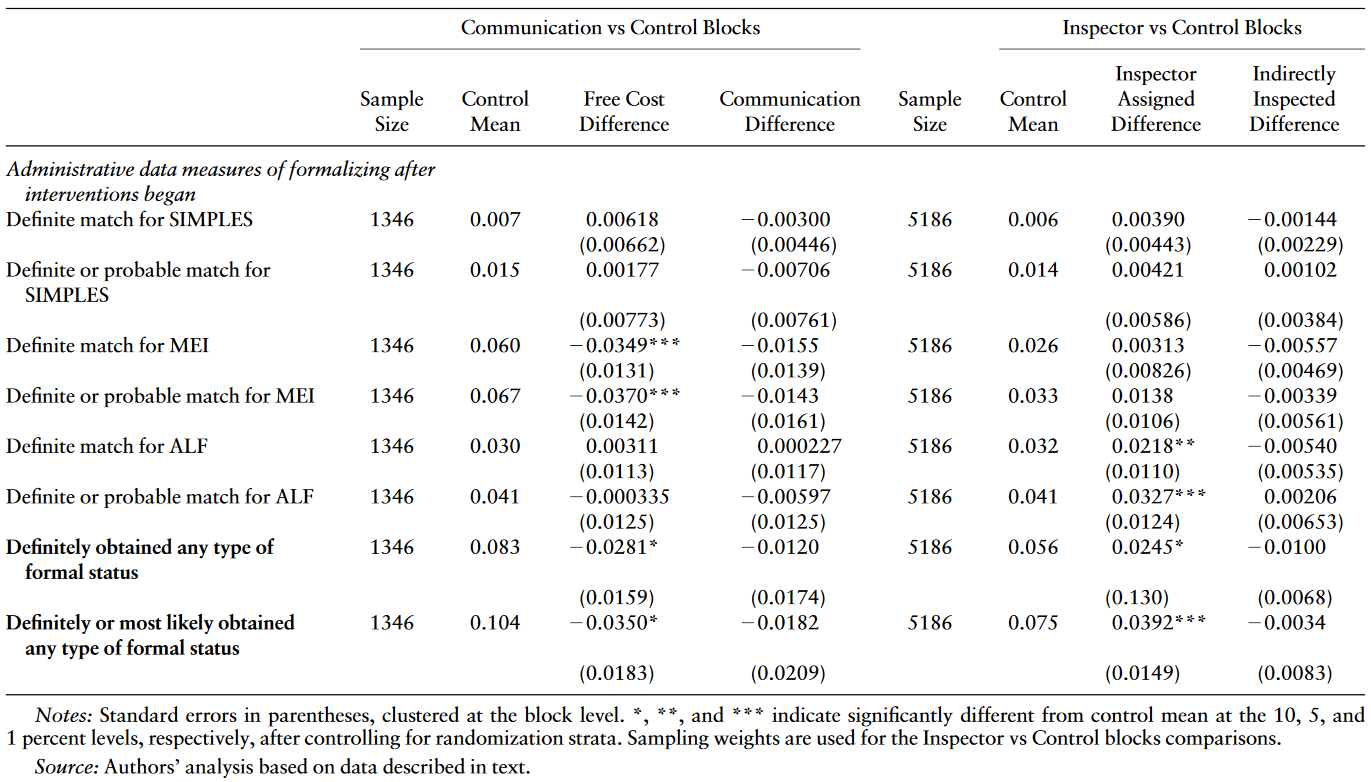
\includegraphics[width=5in]{images/ch6/addition registration fee waiving RCT in brazil.png}
            \caption{Impacts on Formality (\cite{de_andrade_helping_2014})}
            \label{fig:rct brazil result}
        \end{figure}
        
    \subsection{Caveats When Evaluating Those Empirical Studies}
        RCTs, if correctly carried out, have no concerns about endogeneity by design, but this does not mean that RCT results can be apllied anywhere. Common problems of RCTs are:
        \begin{itemize}
            \item RCTs are costly, so typically researchers can only obtain a \emph{small sample}. This casts doubts on the external validity and general equilibrium effects of RCT results
            \item There could be \emph{multiple equilibria} in an economy, depending on the level of informality, trust on government, etc.
            \item A \emph{pre-analysis plan} is ideal to prevent data snooping, but it also confines the potential findings of researches.
        \end{itemize}
